\section{Ranking}\label{ch5}
The topic of \textbf{ranking} is central in the usage of massive data, for example is used in:

\begin{itemize}
    \item \textbf{Search}: a search engine takes a query and provides the most relevant pages on the web in an ordered list;
    \item \textbf{Question answering}: find a resource that contains the answer to a question. QA in turns can be divided into \textit{Factoid QA}, whose goal is to find the answer to a factual question (e.g. "The heigth of Monte Bianco"), and \textit{Community QA}, whose goal is to provide similar questions that other asked in the past;
    \item \textbf{Recommendation}: find new content I might be interested in;
    \item etc..
\end{itemize}

To tackle the problem of document retrieval, many heuristic ranking models have been proposed and used in IR literature. Recently, given the amount of potential training data available, it has become possible to leverage \textbf{Machine Learning (ML)} technologies to build \textbf{effective ranking models}. Specifically, we call those methods that learn how to combine predefined features for ranking by means of discriminative learning \textbf{“learning-to-rank” methods}.

\subsection{What is ranking}
In general, the problem of ranking can be formalized as follows: given a query $q \in Q$ and a (dynamic) collection of documents $D$, ranking finds a \textbf{ordered $k$-subset} that \textbf{maximizes} a function $f : Q \times D^k \to \mathbb{R}^k$.

\begin{figure}[h!]
		\centering
		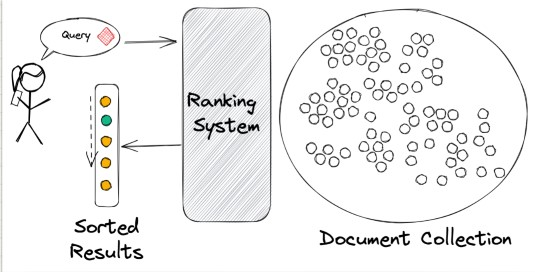
\includegraphics[scale = 1.6]{img/ranking.jpg}
        \label{ranking}
        \caption{Sketch of the ranking problem}
\end{figure}

In general, the main challenges when we talk about ranking are:

\begin{itemize}
    \item How do we evaluate a ranking system?
    \item How do we represent $Q$ and $D$?
    \item What utility do we care about? How do we formulate $f$?
    \item How do we find the $k$-subset from a large collection $D$ as efficiently as possible?
\end{itemize}

Over a decade ago, machine learning transformed how we approach the document ranking problem and answer the questions above. That wave resulted in a paradigm shift from early statistical methods, heuristics, and hand-crafted rules to determine the relevance of documents to a query, to what would later be called \textbf{Learning to Rank} (\textbf{LtR}), where the relevance of a document to a query is estimated by a learnt function, hence “learning” to rank. More specifically, this framework comprises of two distinct algorithms, depicted in Picture \ref{ltr}: \textbf{top-$k$ retrieval}, which finds a subset of $k$ documents that are more relevant to a query, followed by \textbf{ranking} which orders the documents in the top-$k$ set.

\begin{figure}[h!]
		\centering
		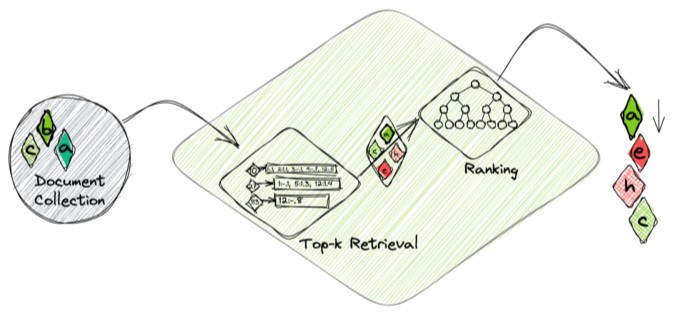
\includegraphics[scale = 1.6]{img/LtR framework.jpg}
        \label{ltr}
        \caption{Top-$k$ retrieval and ranking}
\end{figure}

Usually, the \textbf{ranking stage} uses an often \textbf{expensive function} that was trained using supervised or online learning methods, while the \textbf{retrieval algorithm} solves a form of the \textbf{maximum inner product search (MIPS)} problem among the documents and the queries.

\subsection{LtR framework and approaches}

In general, the following elements are needed to learn a function:

\begin{itemize}
    \item $\Psi$, a \textit{dataset} of labeled examples;
    \item $U(.,.)$, an \textit{evaluation metric};
    \item $l(.,.)$, a \textit{loss function};
    \item $\phi(.)$, a \textit{representation function};
    \item  $f(., \theta)$, the \textit{hypothesis class}, i.e. the relationship between the data and the labels.
\end{itemize}

\begin{figure}[h!]
		\centering
		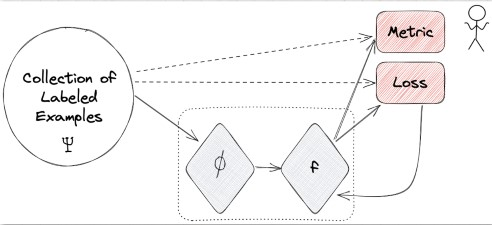
\includegraphics[scale = 1.5]{img/learning a function.jpg}
        \label{learning}
        \caption{Elements to learn a function}
\end{figure}

Moreover, there exist many approaches for LTR framework:

\begin{itemize}
    \item \textbf{Pointwise}: in this case \textbf{each} query-document \textbf{pair} is associated with a \textbf{score}, and the \textbf{objective} of the ML model is to \textbf{predict} such \textbf{score}. In this sense, it can be considered ad a pure \textbf{regression problem} (if the score is "continuous"), or a \textbf{multi-class classification problem} (if the score is "discrete"). Notice that this approach does not consider the position of a document into the final ranking;
    \item \textbf{Pairwise}: in this case we're given \textbf{pairwise preferences}, e.g. $d_1$ is better than $d_2$ for a query $q$, so the \textbf{objective} is to \textbf{predict} a \textbf{score} that \textbf{preserves such preferences}. In this sense, it can be considered as a \textbf{binary classification problem}. Notice that this approach does not consider the relevance of a document into the final ranking;
    \item \textbf{Listwise}: finally, in this case we're given the \textbf{ideal ranking} of results for each query, so the \textbf{objective} is to \textbf{maximize the quality of the whole resulting ranked list} by exploiting the whole list at training time. This approach is also used in recommendation systems.
\end{itemize}

In general, a modern ranking architecture should be:

\begin{itemize}
    \item \textbf{Effective}, i.e. the users should be happy of the results they receive;
    \item \textbf{Efficient}, i.e. it should have a low response time (<0.1 sec);
    \item \textbf{Easy to adapt}, i.e. it should perform a continuous crawling of the Web, exploiting users' feedback.
\end{itemize}


\subsection{Review of Supervised Learning}
The first topic of supervised learning we cover is \textbf{linear regression}. Given $m$ data points $X \in \mathbb{R}^{m \times n}$ and their real values $Y \in \mathbb{R}^m$, we can predict the value of an \textit{unseen} example $x \in \mathbb{R}^n$ using a linear function:

$$
f(x) = w^Tx + b
$$

\begin{figure}[h!]
		\centering
		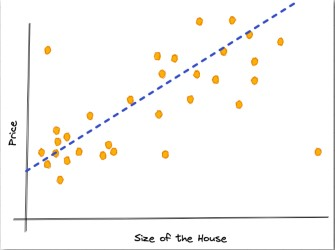
\includegraphics[scale = 1.6]{img/linear regression.jpg}
        \label{linear regression}
        \caption{Linear regression}
\end{figure}

In this case, the \textbf{quality} of the regression function is computed using the \textbf{distance} between the \textbf{predicted value} and the \textbf{actual value}. In particular, many measures exist:

\begin{itemize}
    \item \textit{L1 distance}: $l(f,y) = |f(x) - y|$;
    \item \textit{L2 distance}: $l(f,y) = (f(x) - y)^2$.
\end{itemize}

\begin{figure}[h!]
		\centering
		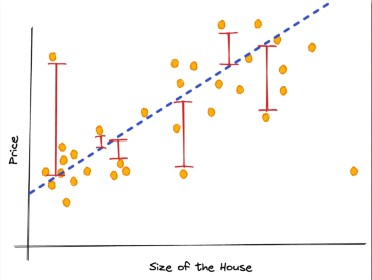
\includegraphics[scale = 1.6]{img/linear regression quality.jpg}
        \label{linear regression quality}
        \caption{Quality of a linear regression function}
\end{figure}

By exploiting this concept of quality of a function, we can \textbf{learn} a regression function by adjusting the parameters of the function, $w \in \mathbb{R}^n$ and $b \in \mathbb{R}$ until the error is minimal. Mathematically, this is translated into the following problem:

$$
w^*,b^* = \text{arg}\min_{w,b} \quad L(f,y) = \text{arg}\min_{w,b} \quad \frac{1}{m} \sum \limits_{i = 1}^m l(f(x_i), y_i)
$$

In particular, the \textit{gradient descent} approach exploits the gradients in order to update the parameters, in particular:

\begin{enumerate}
    \item $w$ and $b$ are initialized randomly;
    \item $$
            w \xleftarrow{} w - \eta \nabla_{w} L(f,y)
            $$
            and
            $$
            b \xleftarrow{} b - \eta \nabla_{b} L(f,y)
            $$
    \item Return $w$ and $b$.
\end{enumerate}

In general, if we have a parameterized function $f(.; \Theta) : \mathbb{R}^n \to \mathbb{R}$, then:

\begin{enumerate}
    \item Initialize $\Theta$ randomly;
    \item Update until convergence:
    $$
    \Theta \xleftarrow{} \Theta - \eta \nabla_{\Theta} L(f(.;\Theta), y)
    $$
    \item Return $\Theta$.
\end{enumerate}

The other important task in Supervised Learning is \textbf{classification}. In this case, the \textit{gradient descent} approach is applied to learn a function $f(.;\Theta) : \mathbb{R} \to \{ \pm 1 \}$. In this case, there exist many different methods for evaluating the accuracy of the predicted class:

\begin{enumerate}
    \item \textit{0-1 loss}:
    $$
    l(f,y) = \begin{cases}
	0 \qquad \text{if } y = f(x)\\
	1 \qquad \text{otherwise} 
	\end{cases}
    $$

    Notice that the problem with this loss is that it cannot be derived!
    
    \item \textit{Hinge loss}:
    $$
    l(f,y) = \text{max} (1 - y(f(x)), 0)
    $$
    \begin{figure}[h!]
		\centering
		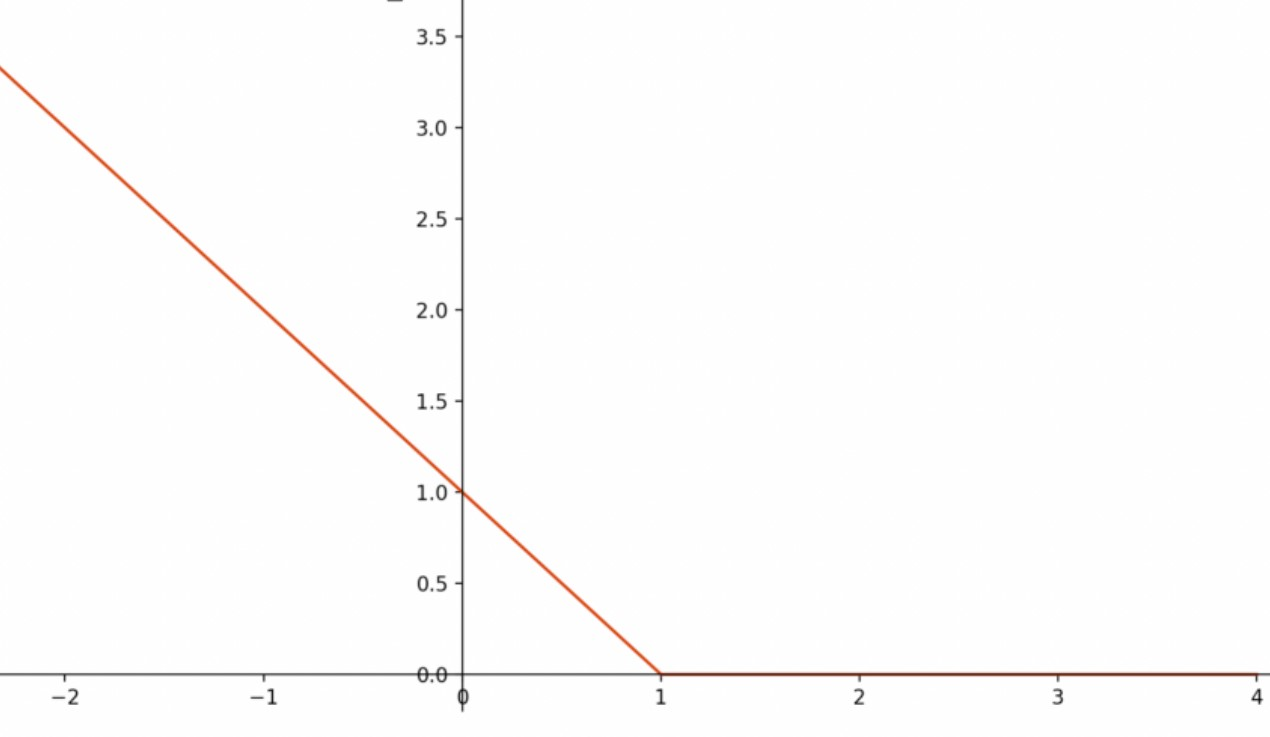
\includegraphics[scale = 0.5]{img/hinge loss.jpg}
        \label{hinge loss}
        \caption{Hinge loss}
    \end{figure}

    \item \textit{Logistic loss}, if $y \in \{ 0,1 \}$:
    $$
    l(f,y) = -y \log \frac{1}{1 + \exp{-f(x)}} - (1-y) \log (1 - \frac{1}{1 + \exp{-f(x)}})
    $$

    \begin{figure}[h!]
		\centering
		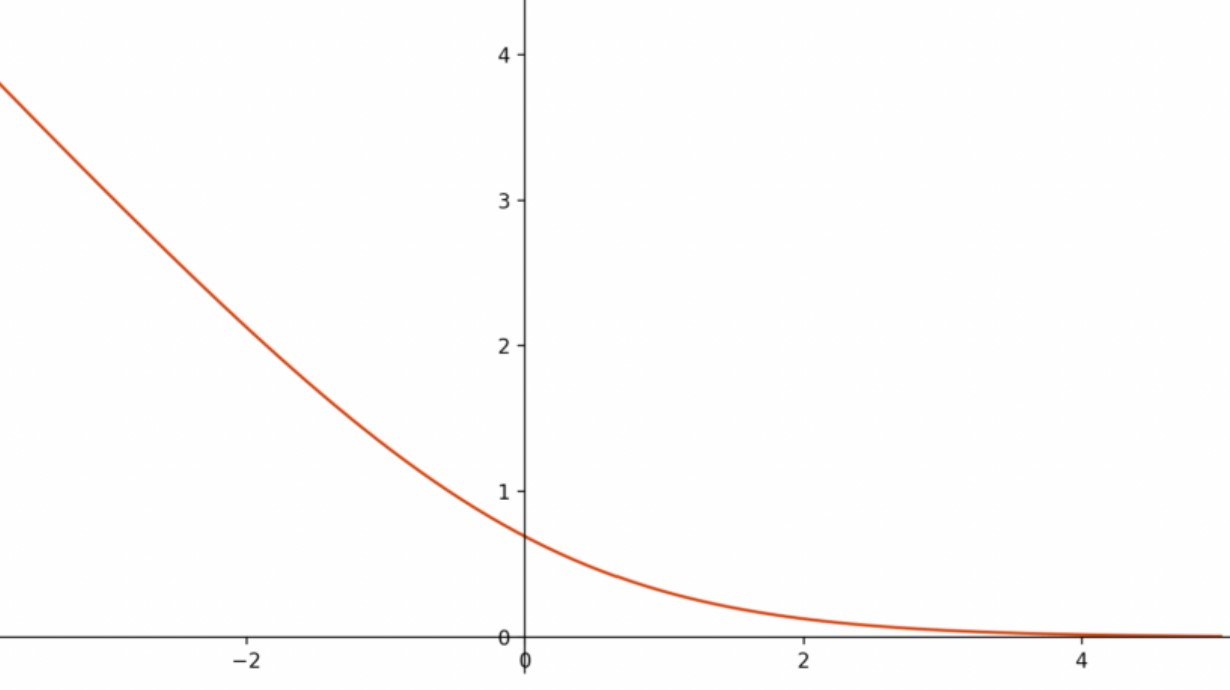
\includegraphics[scale = 0.5]{img/logistic loss.jpg}
        \label{logistic loss}
        \caption{Logistic loss}
    \end{figure}
    
\end{enumerate}

\subsection{Datasets}

A typical LtR dataset comprises a set of triplets $(q,d,y)$, where:

\begin{itemize}
    \item $q \in Q$ represents a \textbf{query} ;
    \item $d \in D$ represents a set of $k$ \textbf{documents} ;
    \item $y \in Y^k$ represents the \textbf{labels} (i.e. the relevance) of the documents.
\end{itemize}

\begin{figure}[h!]
		\centering
		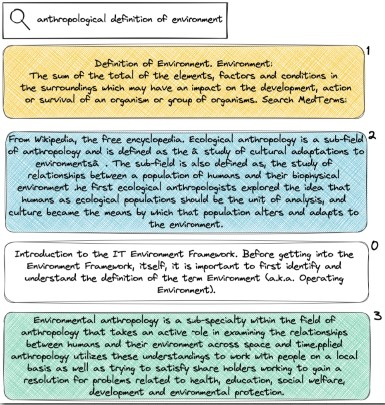
\includegraphics[scale = 1.5]{img/ranking datasets.jpg}
        \label{ranking datasets}
        \caption{Ranking datasets}
\end{figure}

As we can see, this task is more complicated than a classification/regression, since we have multidimensional vectors, and in general the evaluation function is more complicated.

\subsubsection{Representation}
One of the main \textbf{challenges} of ranking datasets is the \textbf{representation of queries and documents}. Suppose for now that there exists a function $\phi : Q \times D \to \mathbb{R}^{k \times m}$, that turns a query and a set of $k$ documents into $m$-dimensional vectors, as represented in Picture \ref{ranking repr}. 

\begin{figure}[h!]
		\centering
		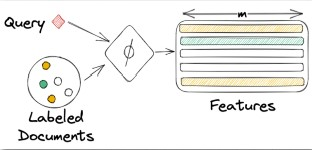
\includegraphics[scale = 2.0]{img/ranking representation.jpg}
        \label{ranking repr}
        \caption{Representation of queries and documents}
\end{figure}

However, we distinguish three methods for selecting the features that represent queries and documents as vectors:

\begin{itemize}
    \item \textbf{query-only features}, for example \textit{query type, length, topic} etc.. These kind of features are only considered for queries;
    \item \textbf{query-independent features}, for example \textit{PageRank, URL, length, in- and out-links, click count} etc.. These kind of features are only considered for documents;
    \item \textbf{query-dependent features}, for example \textit{#query terms, TF-IDF score, BM25 score} etc.. These features are considered for both queries and documents.
\end{itemize}

\subsubsection{Relevance labels}
Regarding the entities involved in the ranking task, the labels may come from:

\begin{itemize}
    \item \textit{explicit feedback}, i.e. human assessors are presented with a query and a ranked list, and they're asked to grade each document w.r.t. the query. Clearly, this approach is not scalable when the collection of documents becomes very large. Moreover, this approach is characterized by several issues: for example, the cost of annotating queries and ranked lists, or the possibility that a new ranking function returns a document which is not judged etc..;
    \item \textit{implicit feedback}, i.e. the users interacting with the ranking system collect signals that are indicative of the relevance of the documents. One the one hand, this approach is scalable, but on the other it may suffer from some biases, e.g. the position bias (users more likely click on the first results). 
\end{itemize}

\subsection{Evaluation metrics}
Another important issue about ranking are the \textbf{ranking metrics}, which are used to evaluate the quality of a ranking. As represented in Picture \ref{ranking metr}, after applying the function $f$ to the vector representation of the documents and the query, for each document we obtain a vector of \textbf{scores} $s \in \mathbb{R}^k$, which in turn is sorted to obtain the ranking $\pi_s$, i.e. the \textbf{actual ranking}. Finally, the actual ranking is compared with the \textbf{ideal ranking} (given by the sorting of the documents in decreasing order of their relevance labels) by using the ranking metrics.

\begin{figure}[h!]
		\centering
		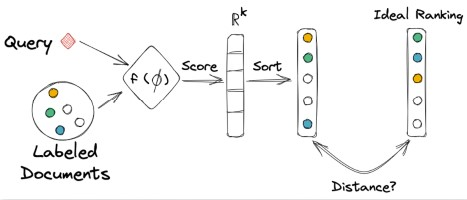
\includegraphics[scale = 2.0]{img/ranking metrics.jpg}
        \label{ranking metr}
        \caption{Evaluation of a ranking function}
\end{figure}

It is helpful to consider the important factors in the way users interact with a ranked list. First, \textbf{users} \textbf{expect} the \textbf{relative ordering of documents to be correct}. That is, documents that are placed higher in the ranked list (i.e., towards the top of the list) should satisfy the information needs of a user better than documents lower on the list, and that as the user goes down the list, documents become less relevant to the query. Second, user \textbf{attention} has a \textbf{skewed distribution} with much of it focused on the top of the ranked list. In other words, users typically do not examine all documents at every position with equal probability or care. As such, higher positions carry more weight.

Some examples of ranking metrics are:

\begin{itemize}
    \item \textit{0-1 loss}, i.e.
    $$
    l(f,y) = \begin{cases}
	0 \qquad \text{if } y = f(x)\\
	1 \qquad \text{otherwise} 
	\end{cases}
    $$
    As we can see, this metric returns 0 if the sorted scores of the actual ranking ($\pi_{f(q,d)}$) are the same of the ones of the ideal ranking ($\pi_y$), 1 otherwise;
    \item \textit{Regression loss}, i.e.
    $$
    l(f,y) = ||f(q,d) - y||_2^2
    $$
    As we can see, this metric measures the squared distance between the actual scores and the ideal scores.
\end{itemize}

However, these two metrics have some disadvantages. The \textit{0-1 loss}, for example, tells us if a ranked list is correct, in its entirety, or not. That's often \textbf{too coarse}. We often don't care how non-relevant documents are ranked with respect to one another, only that relevant documents are above non-relevant ones. That is, if document A is relevant, B, C, and D are not, then A-B-C-D is correct and so is A-C-B-D, but the 0-1 metric considers one of these correct and the other incorrect. On the other hand, a regression loss evaluates whether the ranking function predicted the label of a document (0, 1, 2, etc.). But labels are only used in an ordinal sense: 1 does not mean integer 1, it just indicates a document labeled as 1 is more relevant than a document labeled as 0. So predicting the labels makes little sense.

In this sense, we can introduce some other metrics:

\begin{itemize}
    \item \textit{Kendall's $\tau$}, i.e.:

    $$
    \tau = \frac{2}{n(n-1)} \sum_{i<j} sign(y_i - y_j) sign(f_i - f_j)
    $$

    , which can also be reformulated as:

    $$
    \tau = \frac{\text{(number of concordant pairs) - (number of discordant pairs)}}{\text{number of pairs}}
    $$

    In this sense, the \textit{Kendall's $\tau$} captures the misclassification rate. If we consider, for example, the actual ranking and the ideal ranking in Picture \ref{ranking metr}, then $\tau = \frac{5 - 5}{10}$, since the concordant and discordant pairs are the one represented in Picture \ref{kendall}.

    \begin{figure}[h!]
		\centering
		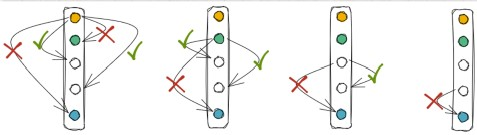
\includegraphics[scale = 2.0]{img/kendall's tau.jpg}
        \label{kendall}
        \caption{Concordant and discordant pairs of Kendall's $\tau$ coefficient}
    \end{figure}

    The main drawback of this metric is that the top and the bottom elements of the ranking are treated equally, while we know that they have different importance.

    \item \textit{ReciprocalRank@k} or \textit{RR@k}, which is defined as the inverse of the rank of the first positive document, i.e. the first document among the top-k of the ranking which has the same ranking in the ideal ranking. If none of the top-k ranked documents is contained in the ideal ranking, the reciprocal rank is 0.

    $$
    RR@k = \frac{1}{\text{rank}_i}
    $$

    \begin{figure}[h!]
		\centering
		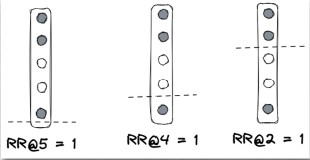
\includegraphics[scale = 2.0]{img/rr@k.jpg}
        \label{rr}
        \caption{RR@k}
    \end{figure}

    The main drawback of this metric is that we only care about the first relevant document, and this is showed in the Picture \ref{rr}, where the RR has the same values for all the values of $k$, since the ranking of the first relevant document is 1.

    \item \textit{Precision@k} or \textit{P@K}, which is defined as the fraction of documents $x_i$ in the top $k$ set for which $y_i > 0$, i.e. the fraction of documents in the top $k$ that are relevant.

    \begin{figure}[h!]
		\centering
		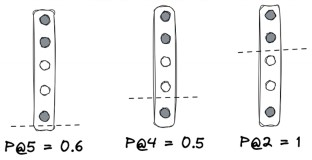
\includegraphics[scale = 2.0]{img/p@k.jpg}
        \label{prec}
        \caption{P@k}
    \end{figure}

    The two main drawbacks of this metric are that it does not take into account the order of the documents, but it only considers the fraction of relevant doc, and tho other issue is that when $k \to \infty$, then $P@k \to 0$, which in general is not a good behaviour.

    \item \textit{Recall@k} or \textit{R@k}, which is defined as the proportion of relevant documents that are retrieved in the first k positions. 
    
    This metric is quite useful, since it can be combined together with the \textit{P@k} metric to produce the \textit{Precision-Recall curve}, for which we can compute AUC. An example is provided in Picture \ref{auc}.

    \begin{figure}[h!]
		\centering
		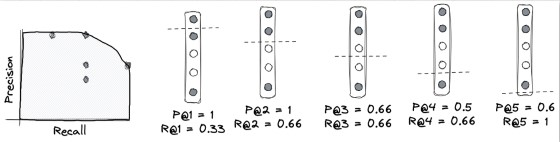
\includegraphics[scale = 2.0]{img/AUC.jpg}
        \label{auc}
        \caption{Precision-Recall curve}
    \end{figure}

    \item \textit{AveragePrecision@k} or \textit{AP@k}, which combines \textit{R@k} and \textit{P@k}:

    $$
    AP@k = \frac{1}{\sum_i \mathbm{1}_{y_{\pi_i} > 0}} \sum \limits_{i = 1}^k \mathbm{1}_{y_{\pi_i} > 0} P@i
    $$

    \item \textit{DiscountedCumulativeGain@k} or \textit{DCG@k}, which tries to focus on the behaviour of a user when a ranked list is presented (Picture \ref{dcg}), and

    \begin{figure}[h!]
		\centering
		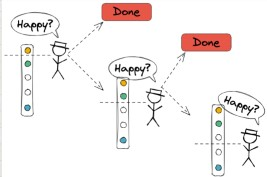
\includegraphics[scale = 2.0]{img/dcg.jpg}
        \label{dcg}
        \caption{Usual behaviour of a user}
    \end{figure}
    
    it is defined as:

    $$
    DCG@k = \sum_{r = 1}^k Gain(y_{\pi_r}) \cdot Discount(r)
    $$
    , where 

    $$
    Gain(y) = 2^y - 1
    $$

    and 
    $$
    Discount(r) = \frac{1}{\log_2(r+1)}
    $$

    We can notice that:

    \begin{itemize}
        \item the input of the \textit{Gain} function is the label of the document in position $r$ of the ranking; if the label is 0, then $Gain = 0$, if the label is 1, then $Gain = 1$;
        \item the \textit{Discount} function is correlated to the probability of a document of being visited.
    \end{itemize}

    \item \textit{NDCG@k}, i.e. the normalization of \textit{DCG@k} by its maximum value.
    
\end{itemize}

In general, by now we've considered only metrics that are related to a single query: given a test set of $N$ ranking samples $\Psi = \{ (q_i, D_i, Y_i) \}_{i = =1}^N $ we can consider the mean of the metrics of interest over the entire set:


    $$
    MAP@k = \frac{1}{N} \sum_i AP@k(\pi_{f(q_i, D_i)}, Y_i)
    $$

    $$
    MeanNDCG@k = \frac{1}{N} \sum_i NDCG@k(\pi_{f(q_i, D_i)}, Y_i)
    $$

, where $\pi_{f(q_i, D_i)}$ denotes the ranked list induced by evaluating $f(q,D)$.

\subsection{Loss functions}
After considering how the dataset is produced and the most important metrics that are used to evaluate a ranking system, we now focus on the \textbf{loss functions}. If we consider again the Picture \ref{learning}, we notice that the loss is used to train our ranking function, and it is used in the training phase.

\begin{figure}[h!]
		\centering
		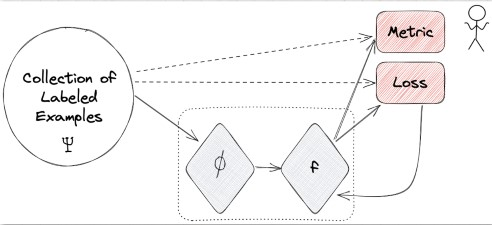
\includegraphics[scale = 1.5]{img/learning a function.jpg}
        \label{learning}
        \caption{Elements to learn a function}
\end{figure}

Depending on the objective of our problem, we may consider many different losses:

\begin{itemize}
    \item If we consider \textbf{ranking} as a \textbf{classification} or \textbf{regression} problem, i.e. each document has a score of relevance (0/1 in case of classification, other scores in case of regression), then we may consider \textbf{pointwise losses}. In this case \textbf{each} query-document \textbf{pair} is associated with a \textbf{score}, and the \textbf{objective} of the ML model is to \textbf{predict} such \textbf{score}. In this sense, it can be considered ad a pure \textbf{regression problem} (if the score is "continuous"), or a \textbf{multi-class classification problem} (if the score is "discrete"). Notice that this approach does not consider the position of a document into the final ranking;

    \item If we consider \textbf{ranking} as a \textbf{preference learning} problem, then we may consider \textbf{pairwise losses}. In this case we're given \textbf{pairwise preferences}, e.g. $d_1$ is better than $d_2$ for a query $q$, so the \textbf{objective} is to \textbf{predict} a \textbf{score} that \textbf{preserves such preferences}. In this sense, it can be considered as a \textbf{binary classification problem}. Notice that this approach does not consider the relevance of a document into the final ranking;
    
    \item If we consider \textbf{ranking} as a \textbf{permutation} or \textbf{probabilistic} problem, then we may consider \textbf{listwise losses}. Finally, in this case we're given the \textbf{ideal ranking} of results for each query, so the \textbf{objective} is to \textbf{maximize the quality of the whole resulting ranked list} by exploiting the whole list at training time. This approach is also used in recommendation systems.
\end{itemize}


\subsubsection{Pointwise losses}

We begin our discussion with the \textbf{regression loss}. In this case:

$$
l(f,y) = ||f(q,d) - y||_2^2
$$

\begin{figure}[h!]
		\centering
		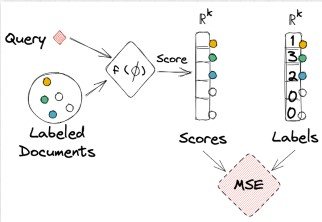
\includegraphics[scale = 2.0]{img/regression losses.jpg}
        \label{regression losses}
        \caption{Regression loss}
\end{figure}

If we consider \textbf{classification loss}, we could either use the \textit{0-1 loss}:

$$
    l(f,y) = \begin{cases}
	0 \qquad \text{if } y = f(x)\\
	1 \qquad \text{otherwise} 
	\end{cases}
$$

or if we assume $f(q,d) = [g(q,d_1), g(q,d_2), .., g(q,d_k)]$ where $g(q,d): Q \times D \to \mathbb{R}$, and given a set of training examples $\Psi = \{ (q_i, d_i, y_i) \}_{i = 1}^N$, then the learning objective becomes the cross entropy:

$$
L(f) = \frac{1}{N} \sum_{(q,d,y) \in \Psi} \sum_{i = 1}^k -y_i \log \frac{1}{1 + e^{-g(q,d_i)}} - (1-y_i) \log [1 - \frac{1}{1 + e^{-g(q,d_i)}}]
$$

, where $\frac{1}{1 + e^{-g(q,d_i)}} = sigmoid(g(q,d_i))$. In this case the gradient of $L$ w.r.t. $g$ is:

$$
\frac{\partial}{\partial g} L(f) = - \frac{1}{N} \sum_{(q,d,y) \in \Psi} \sum_{i = 1}^k (y_i - \frac{1}{1 + e^{-g(q,d_i)}})
$$

Since the \textbf{input} object in the \textbf{pointwise approach} is a \textbf{single document}, the \textbf{relative orde}r between documents \textbf{cannot} be naturally \textbf{considered} in the learning process, although \textbf{ranking} is \textbf{more about predicting relative order} than accurate relevance degree. Moreover, the \textbf{position} of \textbf{each document} in the ranked list is \textbf{invisible} to the \textbf{pointwise loss functions}. Therefore, the pointwise loss function may unconsciously overemphasize those unimportant documents (which are ranked low in the final ranked list and thus do not affect user experiences). 

Given the above problems, the pointwise approach can only be a \textbf{sub-optimal solution to ranking}. To tackle the problem, people have made attempts at regarding a document pair, or the entire group of documents associated with the same query, as the input object. This results in the \textit{pairwise} and \textit{listwise} approaches of learning to rank. With the pairwise approach, the relative order among documents can be better modeled. With the listwise approach, the position information can be visible to the learning-to-rank process.

\subsubsection{Pairwise loss}

If we consider \textbf{pairwise loss}, we could consider Kendall's $\tau$:

$$
\tau = \frac{2}{n(n-1)} \sum_{i<j} sign(y_i - y_j) sign(f_i - f_j)
$$

, which can also be reformulated as:

$$
\tau = \frac{\text{(number of concordant pairs) - (number of discordant pairs)}}{\text{number of pairs}}
$$


Another possibility is to consider \textbf{RankNet's loss function}. 

Assume $f(q,d) = [g(q,d_1), g(q,d_2), .., g(q,d_k)]$ where $g(q,d): Q \times D \to \mathbb{R}$, and given a set of training examples $\Psi = \{ (q_i, d_i, y_i) \}_{i = 1}^N$, then \textit{RankNet}'s learning objective is:

$$
L(f) = \frac{1}{N} \sum_{(q,d,y) \in \Psi} \sum_{i,j} -p_{ij} \log \frac{1}{1 + e^{-(g_i - g_j)}} - p_{ij} \log \frac{1}{1 + e^{-(g_j - g_i)}}
$$
, where $g_i \triangleq g(q,d_i)$, 

$$
p_{ij} = \begin{cases}
	1 \qquad \text{if } y_i > y_j\\
	0.5 \qquad \text{if } y_i = y_j\\
        0 \qquad \text{if } y_i < y_j
	\end{cases}
$$

and 

$$
-p_{ij} \log \frac{1}{1 + e^{-(g_i - g_j)}} - p_{ij} \log \frac{1}{1 + e^{-(g_j - g_i)}} = l_{ij}
$$

In this case the gradient is:

$$
\frac{\partial}{\partial g_i} l_{ij} = -p_{ij} + \frac{1}{1 + e^{-(g_i -g_j)}} = -\frac{\partial}{\partial g_j} l_{ij}
$$

If we denote with $l = \sum_{i,j} l_{ij}$ and let $\Theta$ be the parameters of $g$, we can write:

\begin{equation*}
\begin{split}
\nabla_{\Theta} l = \sum_{i,j} \frac{\partial l_{ij}}{\partial g_i} \nabla_{\Theta} g_i + \frac{\partial l_{ij}}{\partial g_j} \nabla_{\Theta g_j}\\
\qquad = \sum_{i,j} \frac{\partial l_{ij}}{\partial g_i} (\nabla_{\Theta} g_i - \nabla_{Theta} g_j)\\
\qquad = \sum_{i} \left(  \sum_{j : y_i > y_j} \frac{\partial l_{ij}}{\partial g_i} - \sum_{j : y_i < y_j} \frac{\partial l_{ij}}{\partial g_i} \right) \nabla_{\Theta} g_i
\end{split}
\end{equation*}

, where

$$
\sum_{j : y_i > y_j} \frac{\partial l_{ij}}{\partial g_i} - \sum_{j : y_i < y_j} \frac{\partial l_{ij}}{\partial g_i} = \lambda_i
$$

Each $\lambda_i$ can be thought as a force that "pulls" a document down the list of that "pushes" it up the list. We could amplify this force based on the rank of document $d_i$ in the following way:

$$
\nabla_{\Theta l} = \sum_i \left( \sum_{j : y_i > y_j} \frac{\partial l_{ij}}{\partial g_i} |\Delta Z_{ij}| - \sum_{j : y_i < y_j} \frac{\partial l_{ij}}{\partial g_i} |\Delta Z_{ij}| \right)
$$

, where $|\Delta Z_{ij}|$ is the amount of change in the ranking metric $Z$ is $d_i$ and $d_j$ were to trade ranks.

It seems that the pairwise approach has its advantages as compared to the pointwise approach, since it can model the relative order between documents. However, in some cases, it faces even larger challenges than the pointwise approach, for example the problem of the pointwise approach when documents are distributed in an imbalanced manner across queries. Here this issue becomes even more serious in the pairwise approach. Considering that every two documents associated with the same query can create a document pair if their relevance degrees are different, in the worse case, the pair number can be quadratic to the document number. As a result, the difference in the numbers of document pairs is usually significantly larger than the difference in the numbers of documents.

\subsubsection{Listwise loss}

Finally, we can now consider \textbf{listwise loss}: since we cannot directly optimize a \textit{DCG@k} susing gradient descent since it is a discontinuous function, the idea is to replace it with a smooth surrogate, i.e.

$$
DCG@k = \sum_{r \leq k} \frac{2^{y_r} - 1}{\log_2 (\pi^{-1}(d_r) + 1)}
$$

and we can approximate the rank of document $d$ by writing

$$
\pi^{-1}(d_r) = 1 + \sum_{i \neq r} \mathbm{1}_{f_r < f_i} \approx 1 + \sum{i \neq r} \frac{1}{1 + e^{- \alpha (f_i - f_r)}}
$$

Another possibility, provided by the \textbf{ListNet loss function}, is to apply the \textit{softmax} function to both the set of labels $Y$ and to the scores $f(q,d)$. In general, we have that $softmax(x_1) = \frac{e^x_1}{\sum_i e^{x_i}}$, so for $y \in \mathbb{R}^n$ and $f(q,d) \in \mathbb{R}^n$ we have that the \textit{ground truth probability} is:

$$
p_i = \frac{e^{y_i}}{\sum_j e^{y_j}}
$$

, while the \textit{predicted probability} is:

$$
q_i = \frac{e^{f_i}}{\sum_j e^{f_j}}
$$

Finally, we can compute the \textit{cross-entropy} as:

$$
-\sum_i p_i \log q_i
$$

Intuitively speaking, they model the ranking problem in a more natural way than the pointwise and pairwise approaches, and thus can address some problems that these two approaches have encountered. As we have discussed in the previous sections, for the pointwise and pairwise approaches, the position information is invisible to their loss functions, and they ignore the fact that some documents (or document pairs) are associated with the same query. Comparatively speaking, the listwise approach takes all the documents associated with the same query as the input and their ranked list (or their relevance degrees) as the output. In this way, it has the potential to distinguish documents from different queries, and to consider the position information in the output ranked list in its learning process.

\subsection{Ranking functions}
After discussing the loss functions, we now focus on \textbf{ranking functions}. We will mainly focus on three different families of ranking functions:

\begin{itemize}
    \item Gradient Boosting Decision Trees (GBDTs);
    \item Neural Networks and Pre-Trained Transformers;
    \item Inner Product of Dense or Sparse Vectors (or both).
\end{itemize}

\subsubsection{Gradient Boosting Decision Trees (GBDTs)}
In this family of ranking functions we wish to learn an additive function

$$
F^{(M)}(x) = \sum_{t = 1}^M f_t(x)
$$

, where each $f_t(x)$ is a weak learner, that at iteration $m$ learns to predict the residual error:

$$
r_m(x) = - \frac{\partial L(F)}{\partial F}|_{F = F^{m-1}(x)}
$$

The weak learner of GBDTs are the \textbf{regression trees}, which are models that recursively partition the dataset into two subsets by thresholding on a \textit{feature value}: when no further splits are possible, the node of the tree is a \textit{leaf} and it is assigned with the output of the regression. An example is provided in Picture \ref{reg trees}.

\begin{figure}[h!]
		\centering
		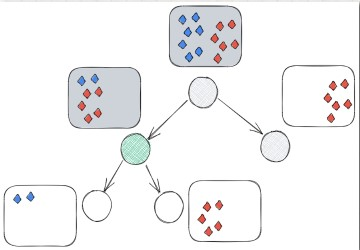
\includegraphics[scale = 1.5]{img/regression trees.jpg}
        \label{reg trees}
        \caption{Regression tree}
\end{figure}

In general, the more leaves, i.e. the more splittings, a regression tree contains, the less generalization in the prediction we have.

Now, we can consider the \textbf{empirical error} of a regression tree $f$ made up of leaves $L_j$ with values $C_j$:

$$
L(f) = \sum_i (y_i - f(x_i))^2 = \sum_{L_j} \sum_{i : x_i \in L_j} (y_i - C_j)^2
$$

, i.e. for each leaf, we compute the squared difference between the actual value and the predicted one.

The \textbf{splitting criterion} of a node $L*$, according to a feature $k*$ and a threshold $\theta*$ is to choose:

$$
L*, k*, \theta* = \arg\min_{L_j, k, \theta} (\min_l \sum_{i : L_j \ni x_{ik} < \theta} (y_i - l)^2 + \min_r \sum_{i : L_j \ni x_{ik} \geq \theta} (y_i - r)^2)
$$

In other words, we want to split the node $L*$, according to a feature $k*$ and a threshold $\theta*$ in a way that minimizes the sum between the empirical error of the left partition and the one of the right partition. The splitting is performed until a stopping criterion is reached, e.g. the number of data points in a leaf is below a certain limit etc..

\subsubsection{Neural Networks and pre-trained Transformers}
One problem of \textit{GBDTs} is that we have to provide ourselves the features to the model, and in general the feature engineering operation is costly. Thus, in this section we focus on the following problem: can we learn $\phi(q,d)$, i.e. the representation of the queries and the documents (possibly in conjunction with $f$)?

For example, \textit{Skip-gram} learns to predict neighboring terms given a current term, or \textit{Continuous Bag of Words} learns to predict a term given its neighboring terms: these methods produce \textbf{static embeddings}. However, there exist some methods that exploit the contextual information in order to represent the words, like \textbf{BERT}.

\subsubsection{Complexity of ranking functions}\label{5.6.3}
In general, the complexity of a ranking system is given by the following costs:

\begin{itemize}
    \item the cost of \textbf{model training};
    \item the cost of \textbf{feature extraction};
    \item the cost of \textbf{model inference}, which may involve hundreds to thousands of decision nodes to traverse or large tensor multiplication.
\end{itemize}

In this section we focus on methods for reducing the inference complexity.

\underline{\textbf{Knowledge distillation}}
The first method we consider is \textbf{knowledge distillation}, which can be described with the following sentence: \textit{given a large model, find a smaller, more efficient model that is just as effective}. In other words, the idea of \textit{knowledge distillation} is to shrink the model in order to produce a more efficient model that is as effective as the original one. 

When considering GBDTs, this technique could be implemented by \textbf{pruning the nodes in the trees}, in order to generate shallower and more balanced trees. For example, we could stop generating nodes when the number of nodes $n \geq \alpha (2^{d+1} - 1)$, where $d$ indicates the depth of the tree. Another techinque could be computing the impact scores of the trees, \textbf{discarding the one with lowest impact}, repeating this operation until $p$ percent of the trees are removed. At each tree discard, the other trees are re-weighted. Finally, one last method could be \textbf{learning a neural network from a tree}, since NNs are more efficient and more predictable.

\underline{\textbf{Early exit algorithm}}
Here, the idea is to perform an approximate inference by stopping the model before its conclusion. 

In the case of GBDTs, we have that:

$$
F(x) = \sum_i f_i(x)
$$

, i.e. the output is the sum of the inference of each decision tree $f_i$, where $x = \phi(q,d) \in \mathbb{R}^m$, as represented in Picture \ref{gdbt}.

\begin{figure}[h!]
		\centering
		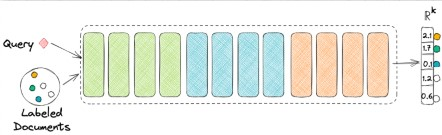
\includegraphics[scale = 2.5]{img/gdbt.jpg}
        \label{gdbt}
        \caption{GBDT for ranking}
\end{figure}

In this sense, the idea of early exit is to compute a "partial" output using a certain number of trees, and then train a classifier that decides whether a document has to be discarded or not, as represented in Picture \ref{gdbt early}. Notice that the decision of discarding a document can rely either on a certain score threshold or on a rank threshold. 

\begin{figure}[h!]
		\centering
		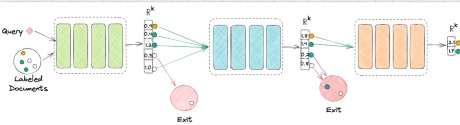
\includegraphics[scale = 2.5]{img/gdbt early exit.jpg}
        \label{gdbt early}
        \caption{GBDT for ranking with early exit}
\end{figure}

A similar method applies for NNs, where a classifier can be inserted in each exit point in order to discard some documents by comparing the current approximate ranking with the ideal one. In this sense, the classifier becomes part of the ranking model, as in the case of GBDT.

\begin{figure}[h!]
		\centering
		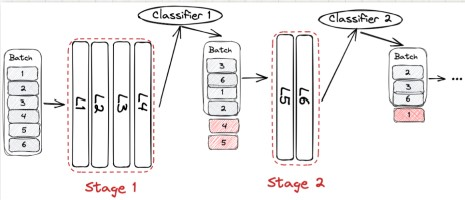
\includegraphics[scale = 2.5]{img/nn exit.jpg}
        \label{nn eaxit}
        \caption{NN with exit points}
\end{figure}

\underline{\textbf{Ranking cascades}}
Thus far we have not considered the case in which a set of documents is provided as input to the ranking model. Due to the dimensionality of the set of documents, applying the same sophisticated ranking function to each of the document becomes very expensive (Picture \ref{rc}): for this reason, the idea of \textbf{ranking cascades} is to apply \textbf{progressively more complex} \textbf{models} to \textbf{progressively smaller} set of \textbf{documents}, as represented in Picture \ref{rc 1}.

\begin{figure}[h!]
		\centering
		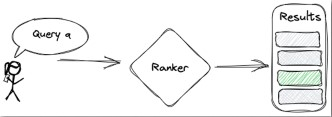
\includegraphics[scale = 2.5]{img/ranking cascades.jpg}
        \label{rc}
        \caption{Normal ranking model}
\end{figure}

\begin{figure}[h!]
		\centering
		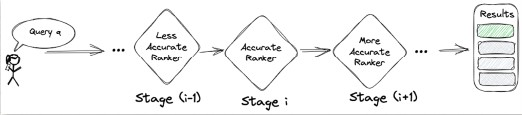
\includegraphics[scale = 2.5]{img/ranking cascades_1.jpg}
        \label{rc 1}
        \caption{Ranking cascade model}
\end{figure}

In this sense, the idea of \textit{ranking cascade} is to use less sophisticated ranking functions to provide faster and less accurate evaluatations on the majority of the documents, and use more sophisticated ranking functions are used to provide more accurate evaluations on few documents. Again, the main idea is that at each evaluation stage some documents are pruned in order to make the evaluation of more sophisticated models feasible in terms of computation time. 

More specifically, 

\begin{enumerate}
    \item Stage $i$ evaluates $f_i(q,d^{(i)})$ on the set of documents $d^{(i)}$;
    \item The set $d^{(i)}$ is pruned and reduced to $d^{(i+1)}$ where $|d^{(i+1)}| \leq |d^{(i)}|$;
    \item $d^{(i)}$ is passed to stage $i+1$.
\end{enumerate}

In this sense, we will see that \textbf{linear functions}, for example \textbf{dot product}, can be used to get rid of the irrelevant documents, in an operation called \textbf{first stage retrieval}.
